%% lyx 2.1.0svn created this file.  For more info, see http://www.lyx.org/.
%% Do not edit unless you really know what you are doing.
\documentclass{article}
\usepackage{graphicx, color}
\newcommand{\hlnumber}[1]{\textcolor[rgb]{0,0,0}{#1}}%
\newcommand{\hlfunctioncall}[1]{\textcolor[rgb]{.5,0,.33}{\textbf{#1}}}%
\newcommand{\hlstring}[1]{\textcolor[rgb]{.6,.6,1}{#1}}%
\newcommand{\hlkeyword}[1]{\textbf{#1}}%
\newcommand{\hlargument}[1]{\textcolor[rgb]{.69,.25,.02}{#1}}%
\newcommand{\hlcomment}[1]{\textcolor[rgb]{.18,.6,.34}{#1}}%
\newcommand{\hlroxygencomment}[1]{\textcolor[rgb]{.44,.48,.7}{#1}}%
\newcommand{\hlformalargs}[1]{\hlargument{#1}}%
\newcommand{\hleqformalargs}[1]{\hlargument{#1}}%
\newcommand{\hlassignement}[1]{\textbf{#1}}%
\newcommand{\hlpackage}[1]{\textcolor[rgb]{.59,.71,.145}{#1}}%
\newcommand{\hlslot}[1]{\textit{#1}}%
\newcommand{\hlsymbol}[1]{#1}%
\newcommand{\hlprompt}[1]{\textcolor[rgb]{.5,.5,.5}{#1}}%

\usepackage{color}%
 
\newsavebox{\hlnormalsizeboxclosebrace}%
\newsavebox{\hlnormalsizeboxopenbrace}%
\newsavebox{\hlnormalsizeboxbackslash}%
\newsavebox{\hlnormalsizeboxlessthan}%
\newsavebox{\hlnormalsizeboxgreaterthan}%
\newsavebox{\hlnormalsizeboxdollar}%
\newsavebox{\hlnormalsizeboxunderscore}%
\newsavebox{\hlnormalsizeboxand}%
\newsavebox{\hlnormalsizeboxhash}%
\newsavebox{\hlnormalsizeboxat}%
\newsavebox{\hlnormalsizeboxpercent}% 
\newsavebox{\hlnormalsizeboxhat}%
\newsavebox{\hlnormalsizeboxsinglequote}%
\newsavebox{\hlnormalsizeboxbacktick}%

\setbox\hlnormalsizeboxopenbrace=\hbox{\begin{normalsize}\verb.{.\end{normalsize}}%
\setbox\hlnormalsizeboxclosebrace=\hbox{\begin{normalsize}\verb.}.\end{normalsize}}%
\setbox\hlnormalsizeboxlessthan=\hbox{\begin{normalsize}\verb.<.\end{normalsize}}%
\setbox\hlnormalsizeboxdollar=\hbox{\begin{normalsize}\verb.$.\end{normalsize}}%
\setbox\hlnormalsizeboxunderscore=\hbox{\begin{normalsize}\verb._.\end{normalsize}}%
\setbox\hlnormalsizeboxand=\hbox{\begin{normalsize}\verb.&.\end{normalsize}}%
\setbox\hlnormalsizeboxhash=\hbox{\begin{normalsize}\verb.#.\end{normalsize}}%
\setbox\hlnormalsizeboxat=\hbox{\begin{normalsize}\verb.@.\end{normalsize}}%
\setbox\hlnormalsizeboxbackslash=\hbox{\begin{normalsize}\verb.\.\end{normalsize}}%
\setbox\hlnormalsizeboxgreaterthan=\hbox{\begin{normalsize}\verb.>.\end{normalsize}}%
\setbox\hlnormalsizeboxpercent=\hbox{\begin{normalsize}\verb.%.\end{normalsize}}%
\setbox\hlnormalsizeboxhat=\hbox{\begin{normalsize}\verb.^.\end{normalsize}}%
\setbox\hlnormalsizeboxsinglequote=\hbox{\begin{normalsize}\verb.'.\end{normalsize}}%
\setbox\hlnormalsizeboxbacktick=\hbox{\begin{normalsize}\verb.`.\end{normalsize}}%
\setbox\hlnormalsizeboxhat=\hbox{\begin{normalsize}\verb.^.\end{normalsize}}%



\newsavebox{\hltinyboxclosebrace}%
\newsavebox{\hltinyboxopenbrace}%
\newsavebox{\hltinyboxbackslash}%
\newsavebox{\hltinyboxlessthan}%
\newsavebox{\hltinyboxgreaterthan}%
\newsavebox{\hltinyboxdollar}%
\newsavebox{\hltinyboxunderscore}%
\newsavebox{\hltinyboxand}%
\newsavebox{\hltinyboxhash}%
\newsavebox{\hltinyboxat}%
\newsavebox{\hltinyboxpercent}% 
\newsavebox{\hltinyboxhat}%
\newsavebox{\hltinyboxsinglequote}%
\newsavebox{\hltinyboxbacktick}%

\setbox\hltinyboxopenbrace=\hbox{\begin{tiny}\verb.{.\end{tiny}}%
\setbox\hltinyboxclosebrace=\hbox{\begin{tiny}\verb.}.\end{tiny}}%
\setbox\hltinyboxlessthan=\hbox{\begin{tiny}\verb.<.\end{tiny}}%
\setbox\hltinyboxdollar=\hbox{\begin{tiny}\verb.$.\end{tiny}}%
\setbox\hltinyboxunderscore=\hbox{\begin{tiny}\verb._.\end{tiny}}%
\setbox\hltinyboxand=\hbox{\begin{tiny}\verb.&.\end{tiny}}%
\setbox\hltinyboxhash=\hbox{\begin{tiny}\verb.#.\end{tiny}}%
\setbox\hltinyboxat=\hbox{\begin{tiny}\verb.@.\end{tiny}}%
\setbox\hltinyboxbackslash=\hbox{\begin{tiny}\verb.\.\end{tiny}}%
\setbox\hltinyboxgreaterthan=\hbox{\begin{tiny}\verb.>.\end{tiny}}%
\setbox\hltinyboxpercent=\hbox{\begin{tiny}\verb.%.\end{tiny}}%
\setbox\hltinyboxhat=\hbox{\begin{tiny}\verb.^.\end{tiny}}%
\setbox\hltinyboxsinglequote=\hbox{\begin{tiny}\verb.'.\end{tiny}}%
\setbox\hltinyboxbacktick=\hbox{\begin{tiny}\verb.`.\end{tiny}}%
\setbox\hltinyboxhat=\hbox{\begin{tiny}\verb.^.\end{tiny}}%



\newsavebox{\hlscriptsizeboxclosebrace}%
\newsavebox{\hlscriptsizeboxopenbrace}%
\newsavebox{\hlscriptsizeboxbackslash}%
\newsavebox{\hlscriptsizeboxlessthan}%
\newsavebox{\hlscriptsizeboxgreaterthan}%
\newsavebox{\hlscriptsizeboxdollar}%
\newsavebox{\hlscriptsizeboxunderscore}%
\newsavebox{\hlscriptsizeboxand}%
\newsavebox{\hlscriptsizeboxhash}%
\newsavebox{\hlscriptsizeboxat}%
\newsavebox{\hlscriptsizeboxpercent}% 
\newsavebox{\hlscriptsizeboxhat}%
\newsavebox{\hlscriptsizeboxsinglequote}%
\newsavebox{\hlscriptsizeboxbacktick}%

\setbox\hlscriptsizeboxopenbrace=\hbox{\begin{scriptsize}\verb.{.\end{scriptsize}}%
\setbox\hlscriptsizeboxclosebrace=\hbox{\begin{scriptsize}\verb.}.\end{scriptsize}}%
\setbox\hlscriptsizeboxlessthan=\hbox{\begin{scriptsize}\verb.<.\end{scriptsize}}%
\setbox\hlscriptsizeboxdollar=\hbox{\begin{scriptsize}\verb.$.\end{scriptsize}}%
\setbox\hlscriptsizeboxunderscore=\hbox{\begin{scriptsize}\verb._.\end{scriptsize}}%
\setbox\hlscriptsizeboxand=\hbox{\begin{scriptsize}\verb.&.\end{scriptsize}}%
\setbox\hlscriptsizeboxhash=\hbox{\begin{scriptsize}\verb.#.\end{scriptsize}}%
\setbox\hlscriptsizeboxat=\hbox{\begin{scriptsize}\verb.@.\end{scriptsize}}%
\setbox\hlscriptsizeboxbackslash=\hbox{\begin{scriptsize}\verb.\.\end{scriptsize}}%
\setbox\hlscriptsizeboxgreaterthan=\hbox{\begin{scriptsize}\verb.>.\end{scriptsize}}%
\setbox\hlscriptsizeboxpercent=\hbox{\begin{scriptsize}\verb.%.\end{scriptsize}}%
\setbox\hlscriptsizeboxhat=\hbox{\begin{scriptsize}\verb.^.\end{scriptsize}}%
\setbox\hlscriptsizeboxsinglequote=\hbox{\begin{scriptsize}\verb.'.\end{scriptsize}}%
\setbox\hlscriptsizeboxbacktick=\hbox{\begin{scriptsize}\verb.`.\end{scriptsize}}%
\setbox\hlscriptsizeboxhat=\hbox{\begin{scriptsize}\verb.^.\end{scriptsize}}%



\newsavebox{\hlfootnotesizeboxclosebrace}%
\newsavebox{\hlfootnotesizeboxopenbrace}%
\newsavebox{\hlfootnotesizeboxbackslash}%
\newsavebox{\hlfootnotesizeboxlessthan}%
\newsavebox{\hlfootnotesizeboxgreaterthan}%
\newsavebox{\hlfootnotesizeboxdollar}%
\newsavebox{\hlfootnotesizeboxunderscore}%
\newsavebox{\hlfootnotesizeboxand}%
\newsavebox{\hlfootnotesizeboxhash}%
\newsavebox{\hlfootnotesizeboxat}%
\newsavebox{\hlfootnotesizeboxpercent}% 
\newsavebox{\hlfootnotesizeboxhat}%
\newsavebox{\hlfootnotesizeboxsinglequote}%
\newsavebox{\hlfootnotesizeboxbacktick}%

\setbox\hlfootnotesizeboxopenbrace=\hbox{\begin{footnotesize}\verb.{.\end{footnotesize}}%
\setbox\hlfootnotesizeboxclosebrace=\hbox{\begin{footnotesize}\verb.}.\end{footnotesize}}%
\setbox\hlfootnotesizeboxlessthan=\hbox{\begin{footnotesize}\verb.<.\end{footnotesize}}%
\setbox\hlfootnotesizeboxdollar=\hbox{\begin{footnotesize}\verb.$.\end{footnotesize}}%
\setbox\hlfootnotesizeboxunderscore=\hbox{\begin{footnotesize}\verb._.\end{footnotesize}}%
\setbox\hlfootnotesizeboxand=\hbox{\begin{footnotesize}\verb.&.\end{footnotesize}}%
\setbox\hlfootnotesizeboxhash=\hbox{\begin{footnotesize}\verb.#.\end{footnotesize}}%
\setbox\hlfootnotesizeboxat=\hbox{\begin{footnotesize}\verb.@.\end{footnotesize}}%
\setbox\hlfootnotesizeboxbackslash=\hbox{\begin{footnotesize}\verb.\.\end{footnotesize}}%
\setbox\hlfootnotesizeboxgreaterthan=\hbox{\begin{footnotesize}\verb.>.\end{footnotesize}}%
\setbox\hlfootnotesizeboxpercent=\hbox{\begin{footnotesize}\verb.%.\end{footnotesize}}%
\setbox\hlfootnotesizeboxhat=\hbox{\begin{footnotesize}\verb.^.\end{footnotesize}}%
\setbox\hlfootnotesizeboxsinglequote=\hbox{\begin{footnotesize}\verb.'.\end{footnotesize}}%
\setbox\hlfootnotesizeboxbacktick=\hbox{\begin{footnotesize}\verb.`.\end{footnotesize}}%
\setbox\hlfootnotesizeboxhat=\hbox{\begin{footnotesize}\verb.^.\end{footnotesize}}%



\newsavebox{\hlsmallboxclosebrace}%
\newsavebox{\hlsmallboxopenbrace}%
\newsavebox{\hlsmallboxbackslash}%
\newsavebox{\hlsmallboxlessthan}%
\newsavebox{\hlsmallboxgreaterthan}%
\newsavebox{\hlsmallboxdollar}%
\newsavebox{\hlsmallboxunderscore}%
\newsavebox{\hlsmallboxand}%
\newsavebox{\hlsmallboxhash}%
\newsavebox{\hlsmallboxat}%
\newsavebox{\hlsmallboxpercent}% 
\newsavebox{\hlsmallboxhat}%
\newsavebox{\hlsmallboxsinglequote}%
\newsavebox{\hlsmallboxbacktick}%

\setbox\hlsmallboxopenbrace=\hbox{\begin{small}\verb.{.\end{small}}%
\setbox\hlsmallboxclosebrace=\hbox{\begin{small}\verb.}.\end{small}}%
\setbox\hlsmallboxlessthan=\hbox{\begin{small}\verb.<.\end{small}}%
\setbox\hlsmallboxdollar=\hbox{\begin{small}\verb.$.\end{small}}%
\setbox\hlsmallboxunderscore=\hbox{\begin{small}\verb._.\end{small}}%
\setbox\hlsmallboxand=\hbox{\begin{small}\verb.&.\end{small}}%
\setbox\hlsmallboxhash=\hbox{\begin{small}\verb.#.\end{small}}%
\setbox\hlsmallboxat=\hbox{\begin{small}\verb.@.\end{small}}%
\setbox\hlsmallboxbackslash=\hbox{\begin{small}\verb.\.\end{small}}%
\setbox\hlsmallboxgreaterthan=\hbox{\begin{small}\verb.>.\end{small}}%
\setbox\hlsmallboxpercent=\hbox{\begin{small}\verb.%.\end{small}}%
\setbox\hlsmallboxhat=\hbox{\begin{small}\verb.^.\end{small}}%
\setbox\hlsmallboxsinglequote=\hbox{\begin{small}\verb.'.\end{small}}%
\setbox\hlsmallboxbacktick=\hbox{\begin{small}\verb.`.\end{small}}%
\setbox\hlsmallboxhat=\hbox{\begin{small}\verb.^.\end{small}}%



\newsavebox{\hllargeboxclosebrace}%
\newsavebox{\hllargeboxopenbrace}%
\newsavebox{\hllargeboxbackslash}%
\newsavebox{\hllargeboxlessthan}%
\newsavebox{\hllargeboxgreaterthan}%
\newsavebox{\hllargeboxdollar}%
\newsavebox{\hllargeboxunderscore}%
\newsavebox{\hllargeboxand}%
\newsavebox{\hllargeboxhash}%
\newsavebox{\hllargeboxat}%
\newsavebox{\hllargeboxpercent}% 
\newsavebox{\hllargeboxhat}%
\newsavebox{\hllargeboxsinglequote}%
\newsavebox{\hllargeboxbacktick}%

\setbox\hllargeboxopenbrace=\hbox{\begin{large}\verb.{.\end{large}}%
\setbox\hllargeboxclosebrace=\hbox{\begin{large}\verb.}.\end{large}}%
\setbox\hllargeboxlessthan=\hbox{\begin{large}\verb.<.\end{large}}%
\setbox\hllargeboxdollar=\hbox{\begin{large}\verb.$.\end{large}}%
\setbox\hllargeboxunderscore=\hbox{\begin{large}\verb._.\end{large}}%
\setbox\hllargeboxand=\hbox{\begin{large}\verb.&.\end{large}}%
\setbox\hllargeboxhash=\hbox{\begin{large}\verb.#.\end{large}}%
\setbox\hllargeboxat=\hbox{\begin{large}\verb.@.\end{large}}%
\setbox\hllargeboxbackslash=\hbox{\begin{large}\verb.\.\end{large}}%
\setbox\hllargeboxgreaterthan=\hbox{\begin{large}\verb.>.\end{large}}%
\setbox\hllargeboxpercent=\hbox{\begin{large}\verb.%.\end{large}}%
\setbox\hllargeboxhat=\hbox{\begin{large}\verb.^.\end{large}}%
\setbox\hllargeboxsinglequote=\hbox{\begin{large}\verb.'.\end{large}}%
\setbox\hllargeboxbacktick=\hbox{\begin{large}\verb.`.\end{large}}%
\setbox\hllargeboxhat=\hbox{\begin{large}\verb.^.\end{large}}%



\newsavebox{\hlLargeboxclosebrace}%
\newsavebox{\hlLargeboxopenbrace}%
\newsavebox{\hlLargeboxbackslash}%
\newsavebox{\hlLargeboxlessthan}%
\newsavebox{\hlLargeboxgreaterthan}%
\newsavebox{\hlLargeboxdollar}%
\newsavebox{\hlLargeboxunderscore}%
\newsavebox{\hlLargeboxand}%
\newsavebox{\hlLargeboxhash}%
\newsavebox{\hlLargeboxat}%
\newsavebox{\hlLargeboxpercent}% 
\newsavebox{\hlLargeboxhat}%
\newsavebox{\hlLargeboxsinglequote}%
\newsavebox{\hlLargeboxbacktick}%

\setbox\hlLargeboxopenbrace=\hbox{\begin{Large}\verb.{.\end{Large}}%
\setbox\hlLargeboxclosebrace=\hbox{\begin{Large}\verb.}.\end{Large}}%
\setbox\hlLargeboxlessthan=\hbox{\begin{Large}\verb.<.\end{Large}}%
\setbox\hlLargeboxdollar=\hbox{\begin{Large}\verb.$.\end{Large}}%
\setbox\hlLargeboxunderscore=\hbox{\begin{Large}\verb._.\end{Large}}%
\setbox\hlLargeboxand=\hbox{\begin{Large}\verb.&.\end{Large}}%
\setbox\hlLargeboxhash=\hbox{\begin{Large}\verb.#.\end{Large}}%
\setbox\hlLargeboxat=\hbox{\begin{Large}\verb.@.\end{Large}}%
\setbox\hlLargeboxbackslash=\hbox{\begin{Large}\verb.\.\end{Large}}%
\setbox\hlLargeboxgreaterthan=\hbox{\begin{Large}\verb.>.\end{Large}}%
\setbox\hlLargeboxpercent=\hbox{\begin{Large}\verb.%.\end{Large}}%
\setbox\hlLargeboxhat=\hbox{\begin{Large}\verb.^.\end{Large}}%
\setbox\hlLargeboxsinglequote=\hbox{\begin{Large}\verb.'.\end{Large}}%
\setbox\hlLargeboxbacktick=\hbox{\begin{Large}\verb.`.\end{Large}}%
\setbox\hlLargeboxhat=\hbox{\begin{Large}\verb.^.\end{Large}}%



\newsavebox{\hlLARGEboxclosebrace}%
\newsavebox{\hlLARGEboxopenbrace}%
\newsavebox{\hlLARGEboxbackslash}%
\newsavebox{\hlLARGEboxlessthan}%
\newsavebox{\hlLARGEboxgreaterthan}%
\newsavebox{\hlLARGEboxdollar}%
\newsavebox{\hlLARGEboxunderscore}%
\newsavebox{\hlLARGEboxand}%
\newsavebox{\hlLARGEboxhash}%
\newsavebox{\hlLARGEboxat}%
\newsavebox{\hlLARGEboxpercent}% 
\newsavebox{\hlLARGEboxhat}%
\newsavebox{\hlLARGEboxsinglequote}%
\newsavebox{\hlLARGEboxbacktick}%

\setbox\hlLARGEboxopenbrace=\hbox{\begin{LARGE}\verb.{.\end{LARGE}}%
\setbox\hlLARGEboxclosebrace=\hbox{\begin{LARGE}\verb.}.\end{LARGE}}%
\setbox\hlLARGEboxlessthan=\hbox{\begin{LARGE}\verb.<.\end{LARGE}}%
\setbox\hlLARGEboxdollar=\hbox{\begin{LARGE}\verb.$.\end{LARGE}}%
\setbox\hlLARGEboxunderscore=\hbox{\begin{LARGE}\verb._.\end{LARGE}}%
\setbox\hlLARGEboxand=\hbox{\begin{LARGE}\verb.&.\end{LARGE}}%
\setbox\hlLARGEboxhash=\hbox{\begin{LARGE}\verb.#.\end{LARGE}}%
\setbox\hlLARGEboxat=\hbox{\begin{LARGE}\verb.@.\end{LARGE}}%
\setbox\hlLARGEboxbackslash=\hbox{\begin{LARGE}\verb.\.\end{LARGE}}%
\setbox\hlLARGEboxgreaterthan=\hbox{\begin{LARGE}\verb.>.\end{LARGE}}%
\setbox\hlLARGEboxpercent=\hbox{\begin{LARGE}\verb.%.\end{LARGE}}%
\setbox\hlLARGEboxhat=\hbox{\begin{LARGE}\verb.^.\end{LARGE}}%
\setbox\hlLARGEboxsinglequote=\hbox{\begin{LARGE}\verb.'.\end{LARGE}}%
\setbox\hlLARGEboxbacktick=\hbox{\begin{LARGE}\verb.`.\end{LARGE}}%
\setbox\hlLARGEboxhat=\hbox{\begin{LARGE}\verb.^.\end{LARGE}}%



\newsavebox{\hlhugeboxclosebrace}%
\newsavebox{\hlhugeboxopenbrace}%
\newsavebox{\hlhugeboxbackslash}%
\newsavebox{\hlhugeboxlessthan}%
\newsavebox{\hlhugeboxgreaterthan}%
\newsavebox{\hlhugeboxdollar}%
\newsavebox{\hlhugeboxunderscore}%
\newsavebox{\hlhugeboxand}%
\newsavebox{\hlhugeboxhash}%
\newsavebox{\hlhugeboxat}%
\newsavebox{\hlhugeboxpercent}% 
\newsavebox{\hlhugeboxhat}%
\newsavebox{\hlhugeboxsinglequote}%
\newsavebox{\hlhugeboxbacktick}%

\setbox\hlhugeboxopenbrace=\hbox{\begin{huge}\verb.{.\end{huge}}%
\setbox\hlhugeboxclosebrace=\hbox{\begin{huge}\verb.}.\end{huge}}%
\setbox\hlhugeboxlessthan=\hbox{\begin{huge}\verb.<.\end{huge}}%
\setbox\hlhugeboxdollar=\hbox{\begin{huge}\verb.$.\end{huge}}%
\setbox\hlhugeboxunderscore=\hbox{\begin{huge}\verb._.\end{huge}}%
\setbox\hlhugeboxand=\hbox{\begin{huge}\verb.&.\end{huge}}%
\setbox\hlhugeboxhash=\hbox{\begin{huge}\verb.#.\end{huge}}%
\setbox\hlhugeboxat=\hbox{\begin{huge}\verb.@.\end{huge}}%
\setbox\hlhugeboxbackslash=\hbox{\begin{huge}\verb.\.\end{huge}}%
\setbox\hlhugeboxgreaterthan=\hbox{\begin{huge}\verb.>.\end{huge}}%
\setbox\hlhugeboxpercent=\hbox{\begin{huge}\verb.%.\end{huge}}%
\setbox\hlhugeboxhat=\hbox{\begin{huge}\verb.^.\end{huge}}%
\setbox\hlhugeboxsinglequote=\hbox{\begin{huge}\verb.'.\end{huge}}%
\setbox\hlhugeboxbacktick=\hbox{\begin{huge}\verb.`.\end{huge}}%
\setbox\hlhugeboxhat=\hbox{\begin{huge}\verb.^.\end{huge}}%



\newsavebox{\hlHugeboxclosebrace}%
\newsavebox{\hlHugeboxopenbrace}%
\newsavebox{\hlHugeboxbackslash}%
\newsavebox{\hlHugeboxlessthan}%
\newsavebox{\hlHugeboxgreaterthan}%
\newsavebox{\hlHugeboxdollar}%
\newsavebox{\hlHugeboxunderscore}%
\newsavebox{\hlHugeboxand}%
\newsavebox{\hlHugeboxhash}%
\newsavebox{\hlHugeboxat}%
\newsavebox{\hlHugeboxpercent}% 
\newsavebox{\hlHugeboxhat}%
\newsavebox{\hlHugeboxsinglequote}%
\newsavebox{\hlHugeboxbacktick}%

\setbox\hlHugeboxopenbrace=\hbox{\begin{Huge}\verb.{.\end{Huge}}%
\setbox\hlHugeboxclosebrace=\hbox{\begin{Huge}\verb.}.\end{Huge}}%
\setbox\hlHugeboxlessthan=\hbox{\begin{Huge}\verb.<.\end{Huge}}%
\setbox\hlHugeboxdollar=\hbox{\begin{Huge}\verb.$.\end{Huge}}%
\setbox\hlHugeboxunderscore=\hbox{\begin{Huge}\verb._.\end{Huge}}%
\setbox\hlHugeboxand=\hbox{\begin{Huge}\verb.&.\end{Huge}}%
\setbox\hlHugeboxhash=\hbox{\begin{Huge}\verb.#.\end{Huge}}%
\setbox\hlHugeboxat=\hbox{\begin{Huge}\verb.@.\end{Huge}}%
\setbox\hlHugeboxbackslash=\hbox{\begin{Huge}\verb.\.\end{Huge}}%
\setbox\hlHugeboxgreaterthan=\hbox{\begin{Huge}\verb.>.\end{Huge}}%
\setbox\hlHugeboxpercent=\hbox{\begin{Huge}\verb.%.\end{Huge}}%
\setbox\hlHugeboxhat=\hbox{\begin{Huge}\verb.^.\end{Huge}}%
\setbox\hlHugeboxsinglequote=\hbox{\begin{Huge}\verb.'.\end{Huge}}%
\setbox\hlHugeboxbacktick=\hbox{\begin{Huge}\verb.`.\end{Huge}}%
\setbox\hlHugeboxhat=\hbox{\begin{Huge}\verb.^.\end{Huge}}%
 

\def\urltilda{\kern -.15em\lower .7ex\hbox{\~{}}\kern .04em}%

\newcommand{\hlstd}[1]{\textcolor[rgb]{0,0,0}{#1}}%
\newcommand{\hlnum}[1]{\textcolor[rgb]{0.16,0.16,1}{#1}}
\newcommand{\hlesc}[1]{\textcolor[rgb]{1,0,1}{#1}}
\newcommand{\hlstr}[1]{\textcolor[rgb]{1,0,0}{#1}}
\newcommand{\hldstr}[1]{\textcolor[rgb]{0.51,0.51,0}{#1}}
\newcommand{\hlslc}[1]{\textcolor[rgb]{0.51,0.51,0.51}{\it{#1}}}
\newcommand{\hlcom}[1]{\textcolor[rgb]{0.51,0.51,0.51}{\it{#1}}}
\newcommand{\hldir}[1]{\textcolor[rgb]{0,0.51,0}{#1}}
\newcommand{\hlsym}[1]{\textcolor[rgb]{0,0,0}{#1}}
\newcommand{\hlline}[1]{\textcolor[rgb]{0.33,0.33,0.33}{#1}}
\newcommand{\hlkwa}[1]{\textcolor[rgb]{0,0,0}{\bf{#1}}}
\newcommand{\hlkwb}[1]{\textcolor[rgb]{0.51,0,0}{#1}}
\newcommand{\hlkwc}[1]{\textcolor[rgb]{0,0,0}{\bf{#1}}}
\newcommand{\hlkwd}[1]{\textcolor[rgb]{0,0,0.51}{#1}}

\definecolor{fgcolor}{rgb}{0,0,0}
\usepackage{framed}
\makeatletter
\newenvironment{kframe}{%
 \def\FrameCommand##1{\hskip\@totalleftmargin \hskip-\fboxsep
 \colorbox{shadecolor}{##1}\hskip-\fboxsep
     % There is no \@totalrightmargin, so:
     \hskip-\linewidth \hskip-\@totalleftmargin \hskip\columnwidth}%
 \MakeFramed {\advance\hsize-\width
   \@totalleftmargin\z@ \linewidth\hsize
   \@setminipage}}%
 {\par\unskip\endMakeFramed}
\makeatother

\newenvironment{knitrout}{}{} % an empty environment to be redefined in TeX

\usepackage[sc]{mathpazo}
\usepackage[T1]{fontenc}
\usepackage{geometry}
\usepackage{amssymb}
\usepackage{amsmath}
\geometry{verbose,tmargin=2.5cm,bmargin=2.5cm,lmargin=2.5cm,rmargin=2.5cm}
\setcounter{secnumdepth}{2}
\setcounter{tocdepth}{2}
\usepackage{url}
\usepackage[unicode=true,pdfusetitle,
 bookmarks=true,bookmarksnumbered=true,bookmarksopen=true,bookmarksopenlevel=2,
 breaklinks=false,pdfborder={0 0 1},backref=false,colorlinks=false]
 {hyperref}
\hypersetup{
 pdfstartview={XYZ null null 1}}
%\usepackage{breakurl}

\makeatletter
%%%%%%%%%%%%%%%%%%%%%%%%%%%%%% User specified LaTeX commands.
\renewcommand{\textfraction}{0.05}
\renewcommand{\topfraction}{0.8}
\renewcommand{\bottomfraction}{0.8}
\renewcommand{\floatpagefraction}{0.75}

\makeatother

\begin{document}

%% still can't get paths to work ...
% 




\begin{center}
  {\bf \Large Homework 4, Statistical Rethinking}\\
\vspace{12pt}
   {\large Jaime Ashander}
\end{center}

We are working with data on urban foxes

\begin{knitrout}
\definecolor{shadecolor}{rgb}{.97, .97, .97}{\color{fgcolor}\begin{kframe}
\begin{flushleft}
\ttfamily\noindent
\hlsymbol{d}{\ }\hlassignement{\usebox{\hlnormalsizeboxlessthan}-}{\ }\hlfunctioncall{read.csv}\hlkeyword{(}\hlstring{"foxes.csv"}\hlkeyword{)}\hspace*{\fill}\\
\hlstd{}\hlfunctioncall{head}\hlkeyword{(}\hlsymbol{d}\hlkeyword{)}\mbox{}
\normalfont
\end{flushleft}
\begin{verbatim}
##   group avgfood groupsize area weight
## 1     1    0.37         2 1.09   5.02
## 2     1    0.37         2 1.09   2.84
## 3     2    0.53         2 2.05   5.33
## 4     2    0.53         2 2.05   6.07
## 5     3    0.49         2 2.12   5.85
## 6     3    0.49         2 2.12   3.25
\end{verbatim}
\end{kframe}}
\end{knitrout}


There are five columns: 
\begin{enumerate}
  \item {\tt group}: Number of the social group the individual fox belongs to. This is just an identify label.
  \item {\tt avgfood}: The average amount of food available in the territory. 
  \item {\tt groupsize}: The number of foxes in the social group. 
  \item {\tt area}: Size of the territory. 
  \item {\tt weight}: Body weight of the individual fox.
\end{enumerate}

\begin{knitrout}
\definecolor{shadecolor}{rgb}{.97, .97, .97}{\color{fgcolor}\begin{kframe}
\begin{flushleft}
\ttfamily\noindent
\hlfunctioncall{cor}\hlkeyword{(}\hlsymbol{d}\hlkeyword{)}\mbox{}
\normalfont
\end{flushleft}
\begin{verbatim}
##             group  avgfood groupsize    area   weight
## group      1.0000  0.34084    0.4010 0.37777 -0.15190
## avgfood    0.3408  1.00000    0.9015 0.88310 -0.02504
## groupsize  0.4010  0.90148    1.0000 0.82759 -0.16099
## area       0.3778  0.88310    0.8276 1.00000  0.01948
## weight    -0.1519 -0.02504   -0.1610 0.01948  1.00000
\end{verbatim}
\end{kframe}}
\end{knitrout}


A glance at the correlation matrix hints that we could be on the look out with problems from correlated predictors.
The tightly corrrelated set of predictors ({\tt avgfood, groupsize, area}) are just on the boundary of correlations where we begin to expect problems ($\approx 90$), so things may work out.

\subsection*{Problem 1}
\label{problem1}

Denoting body weight as $w_i$, territory size $a_i$ (for area), and group size $g_i$, we fit two models: 

(1) modelling body weight as a normal random variable based on area
\[
\begin{split}
w_i \sim {\rm Normal} (\mu_i, \sigma)\\
\mu_i  = \alpha_a + \beta_a a_i
\end{split}
\]


\begin{knitrout}
\definecolor{shadecolor}{rgb}{.97, .97, .97}{\color{fgcolor}\begin{kframe}
\begin{flushleft}
\ttfamily\noindent
\hlsymbol{wa.mle}{\ }\hlassignement{\usebox{\hlnormalsizeboxlessthan}-}{\ }\hlfunctioncall{mle2}\hlkeyword{(}\hlsymbol{weight}{\ }\hlkeyword{\urltilda{}}{\ }\hlfunctioncall{dnorm}\hlkeyword{(}\hlargument{mean}{\ }\hlargument{=}{\ }\hlsymbol{alpha}{\ }\hlkeyword{+}{\ }\hlsymbol{beta}{\ }\hlkeyword{*}{\ }\hlsymbol{area}\hlkeyword{,}\hspace*{\fill}\\
\hlstd{}{\ }{\ }{\ }{\ }\hlargument{sd}{\ }\hlargument{=}{\ }\hlsymbol{sigma}\hlkeyword{)}\hlkeyword{,}{\ }\hlargument{data}{\ }\hlargument{=}{\ }\hlsymbol{d}\hlkeyword{,}{\ }\hlargument{start}{\ }\hlargument{=}{\ }\hlfunctioncall{list}\hlkeyword{(}\hlargument{alpha}{\ }\hlargument{=}{\ }\hlfunctioncall{mean}\hlkeyword{(}\hlsymbol{d}\hlkeyword{\usebox{\hlnormalsizeboxdollar}}\hlsymbol{weight}\hlkeyword{)}\hlkeyword{,}{\ }\hlargument{beta}{\ }\hlargument{=}{\ }\hlnumber{0}\hlkeyword{,}\hspace*{\fill}\\
\hlstd{}{\ }{\ }{\ }{\ }\hlargument{sigma}{\ }\hlargument{=}{\ }\hlfunctioncall{sd}\hlkeyword{(}\hlsymbol{d}\hlkeyword{\usebox{\hlnormalsizeboxdollar}}\hlsymbol{weight}\hlkeyword{)}\hlkeyword{)}\hlkeyword{)}\hspace*{\fill}\\
\hlstd{}\hlsymbol{post}{\ }\hlassignement{\usebox{\hlnormalsizeboxlessthan}-}{\ }\hlfunctioncall{sample.naive.posterior}\hlkeyword{(}\hlsymbol{wa.mle}\hlkeyword{)}\hspace*{\fill}\\
\hlstd{}\hlsymbol{area.rng}{\ }\hlassignement{\usebox{\hlnormalsizeboxlessthan}-}{\ }\hlfunctioncall{seq}\hlkeyword{(}\hlfunctioncall{min}\hlkeyword{(}\hlsymbol{d}\hlkeyword{\usebox{\hlnormalsizeboxdollar}}\hlsymbol{area}\hlkeyword{)}\hlkeyword{,}{\ }\hlfunctioncall{max}\hlkeyword{(}\hlsymbol{d}\hlkeyword{\usebox{\hlnormalsizeboxdollar}}\hlsymbol{area}\hlkeyword{)}\hlkeyword{,}{\ }\hlargument{len}{\ }\hlargument{=}{\ }\hlnumber{1000}\hlkeyword{)}\hspace*{\fill}\\
\hlstd{}\hlsymbol{mu.ci}{\ }\hlassignement{\usebox{\hlnormalsizeboxlessthan}-}{\ }\hlfunctioncall{sapply}\hlkeyword{(}\hlsymbol{area.rng}\hlkeyword{,}{\ }\hlkeyword{function}\hlkeyword{(}\hlformalargs{x}\hlkeyword{)}{\ }\hlkeyword{\usebox{\hlnormalsizeboxopenbrace}}\hspace*{\fill}\\
\hlstd{}{\ }{\ }{\ }{\ }\hlfunctioncall{HPDI}\hlkeyword{(}\hlsymbol{post}\hlkeyword{\usebox{\hlnormalsizeboxdollar}}\hlsymbol{alpha}{\ }\hlkeyword{+}{\ }\hlsymbol{post}\hlkeyword{\usebox{\hlnormalsizeboxdollar}}\hlsymbol{beta}{\ }\hlkeyword{*}{\ }\hlsymbol{x}\hlkeyword{)}\hspace*{\fill}\\
\hlstd{}\hlkeyword{\usebox{\hlnormalsizeboxclosebrace}}\hlkeyword{)}\hspace*{\fill}\\
\hlstd{}\hspace*{\fill}\\
\hlstd{}\hlfunctioncall{plot}\hlkeyword{(}\hlsymbol{weight}{\ }\hlkeyword{\urltilda{}}{\ }\hlsymbol{area}\hlkeyword{,}{\ }\hlargument{data}{\ }\hlargument{=}{\ }\hlsymbol{d}\hlkeyword{)}\hspace*{\fill}\\
\hlstd{}\hlfunctioncall{curve}\hlkeyword{(}\hlfunctioncall{coef}\hlkeyword{(}\hlsymbol{wa.mle}\hlkeyword{)}\hlkeyword{[}\hlstring{"beta"}\hlkeyword{]}{\ }\hlkeyword{*}{\ }\hlsymbol{x}{\ }\hlkeyword{+}{\ }\hlfunctioncall{coef}\hlkeyword{(}\hlsymbol{wa.mle}\hlkeyword{)}\hlkeyword{[}\hlstring{"alpha"}\hlkeyword{]}\hlkeyword{,}{\ }\hlargument{add}{\ }\hlargument{=}{\ }\hlsymbol{T}\hlkeyword{,}\hspace*{\fill}\\
\hlstd{}{\ }{\ }{\ }{\ }\hlargument{from}{\ }\hlargument{=}{\ }\hlfunctioncall{min}\hlkeyword{(}\hlsymbol{d}\hlkeyword{\usebox{\hlnormalsizeboxdollar}}\hlsymbol{area}\hlkeyword{)}\hlkeyword{,}{\ }\hlargument{to}{\ }\hlargument{=}{\ }\hlfunctioncall{max}\hlkeyword{(}\hlsymbol{d}\hlkeyword{\usebox{\hlnormalsizeboxdollar}}\hlsymbol{area}\hlkeyword{)}\hlkeyword{)}\hspace*{\fill}\\
\hlstd{}\hlfunctioncall{lines}\hlkeyword{(}\hlsymbol{mu.ci}\hlkeyword{[}\hlstring{"lower"}\hlkeyword{,}{\ }\hlkeyword{]}{\ }\hlkeyword{\urltilda{}}{\ }\hlsymbol{area.rng}\hlkeyword{,}{\ }\hlargument{data}{\ }\hlargument{=}{\ }\hlsymbol{d}\hlkeyword{,}{\ }\hlargument{lty}{\ }\hlargument{=}{\ }\hlnumber{2}\hlkeyword{)}\hspace*{\fill}\\
\hlstd{}\hlfunctioncall{lines}\hlkeyword{(}\hlsymbol{mu.ci}\hlkeyword{[}\hlstring{"upper"}\hlkeyword{,}{\ }\hlkeyword{]}{\ }\hlkeyword{\urltilda{}}{\ }\hlsymbol{area.rng}\hlkeyword{,}{\ }\hlargument{data}{\ }\hlargument{=}{\ }\hlsymbol{d}\hlkeyword{,}{\ }\hlargument{lty}{\ }\hlargument{=}{\ }\hlnumber{2}\hlkeyword{)}\mbox{}
\normalfont
\end{flushleft}
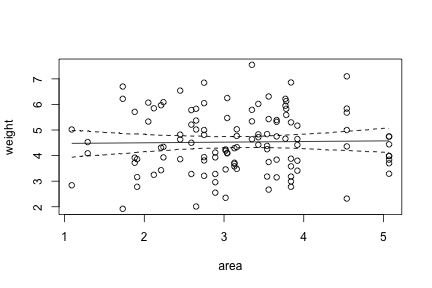
\includegraphics{weight-area} \begin{flushleft}
\ttfamily\noindent
\hlfunctioncall{precis}\hlkeyword{(}\hlsymbol{wa.mle}\hlkeyword{)}\mbox{}
\normalfont
\end{flushleft}
\begin{verbatim}
##       Estimate Std. Error    2.5%  97.5%
## alpha  4.45094    0.39021  3.6861 5.2157
## beta   0.02484    0.11819 -0.2068 0.2565
## sigma  1.17868    0.07738  1.0270 1.3304
\end{verbatim}
\end{kframe}}
\end{knitrout}



(2) modelling body weight as a normal random variable based on group size
\[
\begin{split}
w_i \sim {\rm Normal} (\mu_i, \sigma)\\
\mu_i  = \alpha_g + \beta_g g_i
\end{split}
\]

\begin{knitrout}
\definecolor{shadecolor}{rgb}{.97, .97, .97}{\color{fgcolor}\begin{kframe}
\begin{flushleft}
\ttfamily\noindent
\hlsymbol{wg.mle}{\ }\hlassignement{\usebox{\hlnormalsizeboxlessthan}-}{\ }\hlfunctioncall{mle2}\hlkeyword{(}\hlsymbol{weight}{\ }\hlkeyword{\urltilda{}}{\ }\hlfunctioncall{dnorm}\hlkeyword{(}\hlargument{mean}{\ }\hlargument{=}{\ }\hlsymbol{alpha}{\ }\hlkeyword{+}{\ }\hlsymbol{beta}{\ }\hlkeyword{*}{\ }\hlsymbol{groupsize}\hlkeyword{,}\hspace*{\fill}\\
\hlstd{}{\ }{\ }{\ }{\ }\hlargument{sd}{\ }\hlargument{=}{\ }\hlsymbol{sigma}\hlkeyword{)}\hlkeyword{,}{\ }\hlargument{data}{\ }\hlargument{=}{\ }\hlsymbol{d}\hlkeyword{,}{\ }\hlargument{start}{\ }\hlargument{=}{\ }\hlfunctioncall{list}\hlkeyword{(}\hlargument{alpha}{\ }\hlargument{=}{\ }\hlfunctioncall{mean}\hlkeyword{(}\hlsymbol{d}\hlkeyword{\usebox{\hlnormalsizeboxdollar}}\hlsymbol{weight}\hlkeyword{)}\hlkeyword{,}{\ }\hlargument{beta}{\ }\hlargument{=}{\ }\hlnumber{0}\hlkeyword{,}\hspace*{\fill}\\
\hlstd{}{\ }{\ }{\ }{\ }\hlargument{sigma}{\ }\hlargument{=}{\ }\hlfunctioncall{sd}\hlkeyword{(}\hlsymbol{d}\hlkeyword{\usebox{\hlnormalsizeboxdollar}}\hlsymbol{weight}\hlkeyword{)}\hlkeyword{)}\hlkeyword{)}\mbox{}
\normalfont
\end{flushleft}
\begin{verbatim}
## Warning message: NaNs produced
\end{verbatim}
\begin{flushleft}
\ttfamily\noindent
\hlsymbol{post}{\ }\hlassignement{\usebox{\hlnormalsizeboxlessthan}-}{\ }\hlfunctioncall{sample.naive.posterior}\hlkeyword{(}\hlsymbol{wg.mle}\hlkeyword{)}\hspace*{\fill}\\
\hlstd{}\hlsymbol{groupsize.rng}{\ }\hlassignement{\usebox{\hlnormalsizeboxlessthan}-}{\ }\hlfunctioncall{seq}\hlkeyword{(}\hlfunctioncall{min}\hlkeyword{(}\hlsymbol{d}\hlkeyword{\usebox{\hlnormalsizeboxdollar}}\hlsymbol{groupsize}\hlkeyword{)}\hlkeyword{,}{\ }\hlfunctioncall{max}\hlkeyword{(}\hlsymbol{d}\hlkeyword{\usebox{\hlnormalsizeboxdollar}}\hlsymbol{groupsize}\hlkeyword{)}\hlkeyword{,}\hspace*{\fill}\\
\hlstd{}{\ }{\ }{\ }{\ }\hlargument{len}{\ }\hlargument{=}{\ }\hlnumber{1000}\hlkeyword{)}\hspace*{\fill}\\
\hlstd{}\hlsymbol{mu.ci}{\ }\hlassignement{\usebox{\hlnormalsizeboxlessthan}-}{\ }\hlfunctioncall{sapply}\hlkeyword{(}\hlsymbol{groupsize.rng}\hlkeyword{,}{\ }\hlkeyword{function}\hlkeyword{(}\hlformalargs{x}\hlkeyword{)}{\ }\hlkeyword{\usebox{\hlnormalsizeboxopenbrace}}\hspace*{\fill}\\
\hlstd{}{\ }{\ }{\ }{\ }\hlfunctioncall{HPDI}\hlkeyword{(}\hlsymbol{post}\hlkeyword{\usebox{\hlnormalsizeboxdollar}}\hlsymbol{alpha}{\ }\hlkeyword{+}{\ }\hlsymbol{post}\hlkeyword{\usebox{\hlnormalsizeboxdollar}}\hlsymbol{beta}{\ }\hlkeyword{*}{\ }\hlsymbol{x}\hlkeyword{)}\hspace*{\fill}\\
\hlstd{}\hlkeyword{\usebox{\hlnormalsizeboxclosebrace}}\hlkeyword{)}\hspace*{\fill}\\
\hlstd{}\hspace*{\fill}\\
\hlstd{}\hlfunctioncall{plot}\hlkeyword{(}\hlsymbol{weight}{\ }\hlkeyword{\urltilda{}}{\ }\hlsymbol{groupsize}\hlkeyword{,}{\ }\hlargument{data}{\ }\hlargument{=}{\ }\hlsymbol{d}\hlkeyword{)}\hspace*{\fill}\\
\hlstd{}\hlfunctioncall{curve}\hlkeyword{(}\hlfunctioncall{coef}\hlkeyword{(}\hlsymbol{wg.mle}\hlkeyword{)}\hlkeyword{[}\hlstring{"beta"}\hlkeyword{]}{\ }\hlkeyword{*}{\ }\hlsymbol{x}{\ }\hlkeyword{+}{\ }\hlfunctioncall{coef}\hlkeyword{(}\hlsymbol{wg.mle}\hlkeyword{)}\hlkeyword{[}\hlstring{"alpha"}\hlkeyword{]}\hlkeyword{,}{\ }\hlargument{add}{\ }\hlargument{=}{\ }\hlsymbol{T}\hlkeyword{,}\hspace*{\fill}\\
\hlstd{}{\ }{\ }{\ }{\ }\hlargument{from}{\ }\hlargument{=}{\ }\hlfunctioncall{min}\hlkeyword{(}\hlsymbol{d}\hlkeyword{\usebox{\hlnormalsizeboxdollar}}\hlsymbol{groupsize}\hlkeyword{)}\hlkeyword{,}{\ }\hlargument{to}{\ }\hlargument{=}{\ }\hlfunctioncall{max}\hlkeyword{(}\hlsymbol{d}\hlkeyword{\usebox{\hlnormalsizeboxdollar}}\hlsymbol{groupsize}\hlkeyword{)}\hlkeyword{)}\hspace*{\fill}\\
\hlstd{}\hlfunctioncall{lines}\hlkeyword{(}\hlsymbol{mu.ci}\hlkeyword{[}\hlstring{"lower"}\hlkeyword{,}{\ }\hlkeyword{]}{\ }\hlkeyword{\urltilda{}}{\ }\hlsymbol{groupsize.rng}\hlkeyword{,}{\ }\hlargument{data}{\ }\hlargument{=}{\ }\hlsymbol{d}\hlkeyword{,}{\ }\hlargument{lty}{\ }\hlargument{=}{\ }\hlnumber{2}\hlkeyword{)}\hspace*{\fill}\\
\hlstd{}\hlfunctioncall{lines}\hlkeyword{(}\hlsymbol{mu.ci}\hlkeyword{[}\hlstring{"upper"}\hlkeyword{,}{\ }\hlkeyword{]}{\ }\hlkeyword{\urltilda{}}{\ }\hlsymbol{groupsize.rng}\hlkeyword{,}{\ }\hlargument{data}{\ }\hlargument{=}{\ }\hlsymbol{d}\hlkeyword{,}{\ }\hlargument{lty}{\ }\hlargument{=}{\ }\hlnumber{2}\hlkeyword{)}\mbox{}
\normalfont
\end{flushleft}
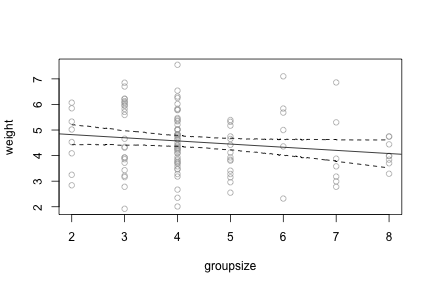
\includegraphics{weight-groupsize} \begin{flushleft}
\ttfamily\noindent
\hlfunctioncall{precis}\hlkeyword{(}\hlsymbol{wg.mle}\hlkeyword{)}\mbox{}
\normalfont
\end{flushleft}
\begin{verbatim}
##       Estimate Std. Error    2.5%   97.5%
## alpha   5.0680    0.32488  4.4312 5.70472
## beta   -0.1239    0.07052 -0.2621 0.01431
## sigma   1.1635    0.07639  1.0138 1.31325
\end{verbatim}
\end{kframe}}
\end{knitrout}


Neither group size (`groupsize`) nor area of territory (`area`) appear to unequivocal predictors of body weight. 
Area seems weakly positive on weight, while group size seems weakly negative. 


\subsection*{Problem 2}
\label{problem2}

Now, modelling body weight as a normal random variable based on group size and area of territory
\[
\begin{split}
w_i \sim {\rm Normal} (\mu_i, \sigma)\\
\mu_i  = \alpha + \beta_g g_i + \beta_a a_i
\end{split}
\]

\begin{knitrout}
\definecolor{shadecolor}{rgb}{.97, .97, .97}{\color{fgcolor}\begin{kframe}
\begin{flushleft}
\ttfamily\noindent
\hlsymbol{wga.mle}{\ }\hlassignement{\usebox{\hlnormalsizeboxlessthan}-}{\ }\hlfunctioncall{mle2}\hlkeyword{(}\hlsymbol{weight}{\ }\hlkeyword{\urltilda{}}{\ }\hlfunctioncall{dnorm}\hlkeyword{(}\hlargument{mean}{\ }\hlargument{=}{\ }\hlsymbol{alpha}{\ }\hlkeyword{+}{\ }\hlsymbol{b.g}{\ }\hlkeyword{*}{\ }\hlsymbol{groupsize}{\ }\hlkeyword{+}\hspace*{\fill}\\
\hlstd{}{\ }{\ }{\ }{\ }\hlsymbol{b.a}{\ }\hlkeyword{*}{\ }\hlsymbol{area}\hlkeyword{,}{\ }\hlargument{sd}{\ }\hlargument{=}{\ }\hlsymbol{sigma}\hlkeyword{)}\hlkeyword{,}{\ }\hlargument{data}{\ }\hlargument{=}{\ }\hlsymbol{d}\hlkeyword{,}{\ }\hlargument{start}{\ }\hlargument{=}{\ }\hlfunctioncall{list}\hlkeyword{(}\hlargument{alpha}{\ }\hlargument{=}{\ }\hlfunctioncall{mean}\hlkeyword{(}\hlsymbol{d}\hlkeyword{\usebox{\hlnormalsizeboxdollar}}\hlsymbol{weight}\hlkeyword{)}\hlkeyword{,}\hspace*{\fill}\\
\hlstd{}{\ }{\ }{\ }{\ }\hlargument{b.g}{\ }\hlargument{=}{\ }\hlnumber{0}\hlkeyword{,}{\ }\hlargument{b.a}{\ }\hlargument{=}{\ }\hlnumber{0}\hlkeyword{,}{\ }\hlargument{sigma}{\ }\hlargument{=}{\ }\hlfunctioncall{sd}\hlkeyword{(}\hlsymbol{d}\hlkeyword{\usebox{\hlnormalsizeboxdollar}}\hlsymbol{weight}\hlkeyword{)}\hlkeyword{)}\hlkeyword{)}\hspace*{\fill}\\
\hlstd{}\hspace*{\fill}\\
\hlstd{}\hspace*{\fill}\\
\hlstd{}\hlsymbol{op}{\ }\hlassignement{\usebox{\hlnormalsizeboxlessthan}-}{\ }\hlfunctioncall{par}\hlkeyword{(}\hlargument{mfrow}{\ }\hlargument{=}{\ }\hlfunctioncall{c}\hlkeyword{(}\hlnumber{1}\hlkeyword{,}{\ }\hlnumber{2}\hlkeyword{)}\hlkeyword{)}\hspace*{\fill}\\
\hlstd{}\hlsymbol{post}{\ }\hlassignement{\usebox{\hlnormalsizeboxlessthan}-}{\ }\hlfunctioncall{sample.naive.posterior}\hlkeyword{(}\hlsymbol{wga.mle}\hlkeyword{)}\hspace*{\fill}\\
\hlstd{}\hspace*{\fill}\\
\hlstd{}\hlcomment{\usebox{\hlnormalsizeboxhash}\usebox{\hlnormalsizeboxhash}{\ }fix{\ }groupsize{\ }and{\ }do{\ }area{\ }effects}\hspace*{\fill}\\
\hlstd{}\hlsymbol{mean.groupsize}{\ }\hlassignement{\usebox{\hlnormalsizeboxlessthan}-}{\ }\hlfunctioncall{mean}\hlkeyword{(}\hlsymbol{d}\hlkeyword{\usebox{\hlnormalsizeboxdollar}}\hlsymbol{groupsize}\hlkeyword{)}\hspace*{\fill}\\
\hlstd{}\hlsymbol{area.rng}{\ }\hlassignement{\usebox{\hlnormalsizeboxlessthan}-}{\ }\hlfunctioncall{seq}\hlkeyword{(}\hlfunctioncall{min}\hlkeyword{(}\hlsymbol{d}\hlkeyword{\usebox{\hlnormalsizeboxdollar}}\hlsymbol{area}\hlkeyword{)}\hlkeyword{,}{\ }\hlfunctioncall{max}\hlkeyword{(}\hlsymbol{d}\hlkeyword{\usebox{\hlnormalsizeboxdollar}}\hlsymbol{area}\hlkeyword{)}\hlkeyword{,}{\ }\hlargument{len}{\ }\hlargument{=}{\ }\hlnumber{1000}\hlkeyword{)}\hspace*{\fill}\\
\hlstd{}\hspace*{\fill}\\
\hlstd{}\hlsymbol{mu.ci}{\ }\hlassignement{\usebox{\hlnormalsizeboxlessthan}-}{\ }\hlfunctioncall{sapply}\hlkeyword{(}\hlsymbol{area.rng}\hlkeyword{,}{\ }\hlkeyword{function}\hlkeyword{(}\hlformalargs{x}\hlkeyword{)}{\ }\hlkeyword{\usebox{\hlnormalsizeboxopenbrace}}\hspace*{\fill}\\
\hlstd{}{\ }{\ }{\ }{\ }\hlfunctioncall{HPDI}\hlkeyword{(}\hlsymbol{post}\hlkeyword{\usebox{\hlnormalsizeboxdollar}}\hlsymbol{alpha}{\ }\hlkeyword{+}{\ }\hlsymbol{post}\hlkeyword{\usebox{\hlnormalsizeboxdollar}}\hlsymbol{b.g}{\ }\hlkeyword{*}{\ }\hlsymbol{mean.groupsize}{\ }\hlkeyword{+}{\ }\hlsymbol{post}\hlkeyword{\usebox{\hlnormalsizeboxdollar}}\hlsymbol{b.a}{\ }\hlkeyword{*}{\ }\hlsymbol{x}\hlkeyword{)}\hspace*{\fill}\\
\hlstd{}\hlkeyword{\usebox{\hlnormalsizeboxclosebrace}}\hlkeyword{)}\hspace*{\fill}\\
\hlstd{}\hlfunctioncall{plot}\hlkeyword{(}\hlsymbol{weight}{\ }\hlkeyword{\urltilda{}}{\ }\hlsymbol{area}\hlkeyword{,}{\ }\hlargument{data}{\ }\hlargument{=}{\ }\hlsymbol{d}\hlkeyword{)}\hspace*{\fill}\\
\hlstd{}\hlfunctioncall{curve}\hlkeyword{(}\hlfunctioncall{coef}\hlkeyword{(}\hlsymbol{wga.mle}\hlkeyword{)}\hlkeyword{[}\hlstring{"b.g"}\hlkeyword{]}{\ }\hlkeyword{*}{\ }\hlsymbol{mean.groupsize}{\ }\hlkeyword{+}{\ }\hlfunctioncall{coef}\hlkeyword{(}\hlsymbol{wga.mle}\hlkeyword{)}\hlkeyword{[}\hlstring{"alpha"}\hlkeyword{]}{\ }\hlkeyword{+}\hspace*{\fill}\\
\hlstd{}{\ }{\ }{\ }{\ }\hlfunctioncall{coef}\hlkeyword{(}\hlsymbol{wga.mle}\hlkeyword{)}\hlkeyword{[}\hlstring{"b.a"}\hlkeyword{]}{\ }\hlkeyword{*}{\ }\hlsymbol{x}\hlkeyword{,}{\ }\hlargument{add}{\ }\hlargument{=}{\ }\hlsymbol{T}\hlkeyword{,}{\ }\hlargument{from}{\ }\hlargument{=}{\ }\hlfunctioncall{min}\hlkeyword{(}\hlsymbol{d}\hlkeyword{\usebox{\hlnormalsizeboxdollar}}\hlsymbol{area}\hlkeyword{)}\hlkeyword{,}{\ }\hlargument{to}{\ }\hlargument{=}{\ }\hlfunctioncall{max}\hlkeyword{(}\hlsymbol{d}\hlkeyword{\usebox{\hlnormalsizeboxdollar}}\hlsymbol{area}\hlkeyword{)}\hlkeyword{)}\hspace*{\fill}\\
\hlstd{}\hspace*{\fill}\\
\hlstd{}\hlfunctioncall{lines}\hlkeyword{(}\hlsymbol{mu.ci}\hlkeyword{[}\hlstring{"lower"}\hlkeyword{,}{\ }\hlkeyword{]}{\ }\hlkeyword{\urltilda{}}{\ }\hlsymbol{area.rng}\hlkeyword{,}{\ }\hlargument{data}{\ }\hlargument{=}{\ }\hlsymbol{d}\hlkeyword{,}{\ }\hlargument{lty}{\ }\hlargument{=}{\ }\hlnumber{2}\hlkeyword{)}\hspace*{\fill}\\
\hlstd{}\hlfunctioncall{lines}\hlkeyword{(}\hlsymbol{mu.ci}\hlkeyword{[}\hlstring{"upper"}\hlkeyword{,}{\ }\hlkeyword{]}{\ }\hlkeyword{\urltilda{}}{\ }\hlsymbol{area.rng}\hlkeyword{,}{\ }\hlargument{data}{\ }\hlargument{=}{\ }\hlsymbol{d}\hlkeyword{,}{\ }\hlargument{lty}{\ }\hlargument{=}{\ }\hlnumber{2}\hlkeyword{)}\hspace*{\fill}\\
\hlstd{}\hspace*{\fill}\\
\hlstd{}\hlcomment{\usebox{\hlnormalsizeboxhash}\usebox{\hlnormalsizeboxhash}{\ }fix{\ }area{\ }and{\ }do{\ }groupsize{\ }effects}\hspace*{\fill}\\
\hlstd{}\hlsymbol{mean.area}{\ }\hlassignement{\usebox{\hlnormalsizeboxlessthan}-}{\ }\hlfunctioncall{mean}\hlkeyword{(}\hlsymbol{d}\hlkeyword{\usebox{\hlnormalsizeboxdollar}}\hlsymbol{area}\hlkeyword{)}\hspace*{\fill}\\
\hlstd{}\hlsymbol{groupsize.rng}{\ }\hlassignement{\usebox{\hlnormalsizeboxlessthan}-}{\ }\hlfunctioncall{seq}\hlkeyword{(}\hlfunctioncall{min}\hlkeyword{(}\hlsymbol{d}\hlkeyword{\usebox{\hlnormalsizeboxdollar}}\hlsymbol{groupsize}\hlkeyword{)}\hlkeyword{,}{\ }\hlfunctioncall{max}\hlkeyword{(}\hlsymbol{d}\hlkeyword{\usebox{\hlnormalsizeboxdollar}}\hlsymbol{groupsize}\hlkeyword{)}\hlkeyword{,}\hspace*{\fill}\\
\hlstd{}{\ }{\ }{\ }{\ }\hlargument{len}{\ }\hlargument{=}{\ }\hlnumber{1000}\hlkeyword{)}\hspace*{\fill}\\
\hlstd{}\hspace*{\fill}\\
\hlstd{}\hlsymbol{mu.ci}{\ }\hlassignement{\usebox{\hlnormalsizeboxlessthan}-}{\ }\hlfunctioncall{sapply}\hlkeyword{(}\hlsymbol{groupsize.rng}\hlkeyword{,}{\ }\hlkeyword{function}\hlkeyword{(}\hlformalargs{x}\hlkeyword{)}{\ }\hlkeyword{\usebox{\hlnormalsizeboxopenbrace}}\hspace*{\fill}\\
\hlstd{}{\ }{\ }{\ }{\ }\hlfunctioncall{HPDI}\hlkeyword{(}\hlsymbol{post}\hlkeyword{\usebox{\hlnormalsizeboxdollar}}\hlsymbol{alpha}{\ }\hlkeyword{+}{\ }\hlsymbol{post}\hlkeyword{\usebox{\hlnormalsizeboxdollar}}\hlsymbol{b.g}{\ }\hlkeyword{*}{\ }\hlsymbol{x}{\ }\hlkeyword{+}{\ }\hlsymbol{post}\hlkeyword{\usebox{\hlnormalsizeboxdollar}}\hlsymbol{b.a}{\ }\hlkeyword{*}{\ }\hlsymbol{mean.area}\hlkeyword{)}\hspace*{\fill}\\
\hlstd{}\hlkeyword{\usebox{\hlnormalsizeboxclosebrace}}\hlkeyword{)}\hspace*{\fill}\\
\hlstd{}\hlfunctioncall{plot}\hlkeyword{(}\hlsymbol{weight}{\ }\hlkeyword{\urltilda{}}{\ }\hlsymbol{groupsize}\hlkeyword{,}{\ }\hlargument{data}{\ }\hlargument{=}{\ }\hlsymbol{d}\hlkeyword{)}\hspace*{\fill}\\
\hlstd{}\hlfunctioncall{curve}\hlkeyword{(}\hlfunctioncall{coef}\hlkeyword{(}\hlsymbol{wga.mle}\hlkeyword{)}\hlkeyword{[}\hlstring{"b.g"}\hlkeyword{]}{\ }\hlkeyword{*}{\ }\hlsymbol{x}{\ }\hlkeyword{+}{\ }\hlfunctioncall{coef}\hlkeyword{(}\hlsymbol{wga.mle}\hlkeyword{)}\hlkeyword{[}\hlstring{"alpha"}\hlkeyword{]}{\ }\hlkeyword{+}\hspace*{\fill}\\
\hlstd{}{\ }{\ }{\ }{\ }\hlfunctioncall{coef}\hlkeyword{(}\hlsymbol{wga.mle}\hlkeyword{)}\hlkeyword{[}\hlstring{"b.a"}\hlkeyword{]}{\ }\hlkeyword{*}{\ }\hlsymbol{mean.area}\hlkeyword{,}{\ }\hlargument{add}{\ }\hlargument{=}{\ }\hlsymbol{T}\hlkeyword{,}{\ }\hlargument{from}{\ }\hlargument{=}{\ }\hlfunctioncall{min}\hlkeyword{(}\hlsymbol{d}\hlkeyword{\usebox{\hlnormalsizeboxdollar}}\hlsymbol{groupsize}\hlkeyword{)}\hlkeyword{,}\hspace*{\fill}\\
\hlstd{}{\ }{\ }{\ }{\ }\hlargument{to}{\ }\hlargument{=}{\ }\hlfunctioncall{max}\hlkeyword{(}\hlsymbol{d}\hlkeyword{\usebox{\hlnormalsizeboxdollar}}\hlsymbol{groupsize}\hlkeyword{)}\hlkeyword{)}\hspace*{\fill}\\
\hlstd{}\hspace*{\fill}\\
\hlstd{}\hlfunctioncall{lines}\hlkeyword{(}\hlsymbol{mu.ci}\hlkeyword{[}\hlstring{"lower"}\hlkeyword{,}{\ }\hlkeyword{]}{\ }\hlkeyword{\urltilda{}}{\ }\hlsymbol{groupsize.rng}\hlkeyword{,}{\ }\hlargument{data}{\ }\hlargument{=}{\ }\hlsymbol{d}\hlkeyword{,}{\ }\hlargument{lty}{\ }\hlargument{=}{\ }\hlnumber{2}\hlkeyword{)}\hspace*{\fill}\\
\hlstd{}\hlfunctioncall{lines}\hlkeyword{(}\hlsymbol{mu.ci}\hlkeyword{[}\hlstring{"upper"}\hlkeyword{,}{\ }\hlkeyword{]}{\ }\hlkeyword{\urltilda{}}{\ }\hlsymbol{groupsize.rng}\hlkeyword{,}{\ }\hlargument{data}{\ }\hlargument{=}{\ }\hlsymbol{d}\hlkeyword{,}{\ }\hlargument{lty}{\ }\hlargument{=}{\ }\hlnumber{2}\hlkeyword{)}\mbox{}
\normalfont
\end{flushleft}
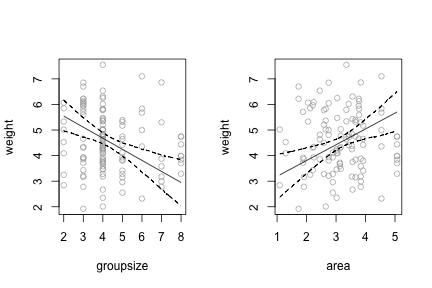
\includegraphics{weight-groupsize-area} \begin{flushleft}
\ttfamily\noindent
\hspace*{\fill}\\
\hlstd{}\hlfunctioncall{par}\hlkeyword{(}\hlsymbol{op}\hlkeyword{)}\hspace*{\fill}\\
\hlstd{}\hspace*{\fill}\\
\hlstd{}\hlfunctioncall{precis}\hlkeyword{(}\hlsymbol{wga.mle}\hlkeyword{)}\mbox{}
\normalfont
\end{flushleft}
\begin{verbatim}
##       Estimate Std. Error    2.5%   97.5%
## alpha   4.4502    0.37087  3.7233  5.1771
## b.g    -0.4326    0.12077 -0.6693 -0.1959
## b.a     0.6182    0.20014  0.2259  1.0104
## sigma   1.1185    0.07343  0.9745  1.2624
\end{verbatim}
\end{kframe}}
\end{knitrout}


Now the estimates are both awesome.
Tight CIs around the mean, clear evidence that as group size increases, weight decreases and that as area increases so does weight. 


\subsection*{Problem 3}
\label{problem3}


Closing the loop \dots 

(1)
Now, modelling body weight as a normal random variable based on group size and average food
\[
\begin{split}
w_i \sim {\rm Normal} (\mu_i, \sigma)\\
\mu_i  = \alpha + \beta_g g_i + \beta_v v_i
\end{split}
\]

\begin{knitrout}
\definecolor{shadecolor}{rgb}{.97, .97, .97}{\color{fgcolor}\begin{kframe}
\begin{flushleft}
\ttfamily\noindent
\hlsymbol{wgv.mle}{\ }\hlassignement{\usebox{\hlnormalsizeboxlessthan}-}{\ }\hlfunctioncall{mle2}\hlkeyword{(}\hlsymbol{weight}{\ }\hlkeyword{\urltilda{}}{\ }\hlfunctioncall{dnorm}\hlkeyword{(}\hlargument{mean}{\ }\hlargument{=}{\ }\hlsymbol{alpha}{\ }\hlkeyword{+}{\ }\hlsymbol{b.g}{\ }\hlkeyword{*}{\ }\hlsymbol{groupsize}{\ }\hlkeyword{+}\hspace*{\fill}\\
\hlstd{}{\ }{\ }{\ }{\ }\hlsymbol{b.v}{\ }\hlkeyword{*}{\ }\hlsymbol{avgfood}\hlkeyword{,}{\ }\hlargument{sd}{\ }\hlargument{=}{\ }\hlsymbol{sigma}\hlkeyword{)}\hlkeyword{,}{\ }\hlargument{data}{\ }\hlargument{=}{\ }\hlsymbol{d}\hlkeyword{,}{\ }\hlargument{start}{\ }\hlargument{=}{\ }\hlfunctioncall{list}\hlkeyword{(}\hlargument{alpha}{\ }\hlargument{=}{\ }\hlfunctioncall{mean}\hlkeyword{(}\hlsymbol{d}\hlkeyword{\usebox{\hlnormalsizeboxdollar}}\hlsymbol{weight}\hlkeyword{)}\hlkeyword{,}\hspace*{\fill}\\
\hlstd{}{\ }{\ }{\ }{\ }\hlargument{b.g}{\ }\hlargument{=}{\ }\hlnumber{0}\hlkeyword{,}{\ }\hlargument{b.v}{\ }\hlargument{=}{\ }\hlnumber{0}\hlkeyword{,}{\ }\hlargument{sigma}{\ }\hlargument{=}{\ }\hlfunctioncall{sd}\hlkeyword{(}\hlsymbol{d}\hlkeyword{\usebox{\hlnormalsizeboxdollar}}\hlsymbol{weight}\hlkeyword{)}\hlkeyword{)}\hlkeyword{)}\hspace*{\fill}\\
\hlstd{}\hspace*{\fill}\\
\hlstd{}\hspace*{\fill}\\
\hlstd{}\hlsymbol{op}{\ }\hlassignement{\usebox{\hlnormalsizeboxlessthan}-}{\ }\hlfunctioncall{par}\hlkeyword{(}\hlargument{mfrow}{\ }\hlargument{=}{\ }\hlfunctioncall{c}\hlkeyword{(}\hlnumber{1}\hlkeyword{,}{\ }\hlnumber{2}\hlkeyword{)}\hlkeyword{)}\hspace*{\fill}\\
\hlstd{}\hlsymbol{post}{\ }\hlassignement{\usebox{\hlnormalsizeboxlessthan}-}{\ }\hlfunctioncall{sample.naive.posterior}\hlkeyword{(}\hlsymbol{wgv.mle}\hlkeyword{)}\hspace*{\fill}\\
\hlstd{}\hspace*{\fill}\\
\hlstd{}\hlcomment{\usebox{\hlnormalsizeboxhash}\usebox{\hlnormalsizeboxhash}{\ }fix{\ }groupsize{\ }and{\ }do{\ }avgfood{\ }effects}\hspace*{\fill}\\
\hlstd{}\hlsymbol{mean.groupsize}{\ }\hlassignement{\usebox{\hlnormalsizeboxlessthan}-}{\ }\hlfunctioncall{mean}\hlkeyword{(}\hlsymbol{d}\hlkeyword{\usebox{\hlnormalsizeboxdollar}}\hlsymbol{groupsize}\hlkeyword{)}\hspace*{\fill}\\
\hlstd{}\hlsymbol{avgfood.rng}{\ }\hlassignement{\usebox{\hlnormalsizeboxlessthan}-}{\ }\hlfunctioncall{seq}\hlkeyword{(}\hlfunctioncall{min}\hlkeyword{(}\hlsymbol{d}\hlkeyword{\usebox{\hlnormalsizeboxdollar}}\hlsymbol{avgfood}\hlkeyword{)}\hlkeyword{,}{\ }\hlfunctioncall{max}\hlkeyword{(}\hlsymbol{d}\hlkeyword{\usebox{\hlnormalsizeboxdollar}}\hlsymbol{avgfood}\hlkeyword{)}\hlkeyword{,}{\ }\hlargument{len}{\ }\hlargument{=}{\ }\hlnumber{1000}\hlkeyword{)}\hspace*{\fill}\\
\hlstd{}\hspace*{\fill}\\
\hlstd{}\hlsymbol{mu.ci}{\ }\hlassignement{\usebox{\hlnormalsizeboxlessthan}-}{\ }\hlfunctioncall{sapply}\hlkeyword{(}\hlsymbol{avgfood.rng}\hlkeyword{,}{\ }\hlkeyword{function}\hlkeyword{(}\hlformalargs{x}\hlkeyword{)}{\ }\hlkeyword{\usebox{\hlnormalsizeboxopenbrace}}\hspace*{\fill}\\
\hlstd{}{\ }{\ }{\ }{\ }\hlfunctioncall{HPDI}\hlkeyword{(}\hlsymbol{post}\hlkeyword{\usebox{\hlnormalsizeboxdollar}}\hlsymbol{alpha}{\ }\hlkeyword{+}{\ }\hlsymbol{post}\hlkeyword{\usebox{\hlnormalsizeboxdollar}}\hlsymbol{b.g}{\ }\hlkeyword{*}{\ }\hlsymbol{mean.groupsize}{\ }\hlkeyword{+}{\ }\hlsymbol{post}\hlkeyword{\usebox{\hlnormalsizeboxdollar}}\hlsymbol{b.v}{\ }\hlkeyword{*}{\ }\hlsymbol{x}\hlkeyword{)}\hspace*{\fill}\\
\hlstd{}\hlkeyword{\usebox{\hlnormalsizeboxclosebrace}}\hlkeyword{)}\hspace*{\fill}\\
\hlstd{}\hlfunctioncall{plot}\hlkeyword{(}\hlsymbol{weight}{\ }\hlkeyword{\urltilda{}}{\ }\hlsymbol{avgfood}\hlkeyword{,}{\ }\hlargument{data}{\ }\hlargument{=}{\ }\hlsymbol{d}\hlkeyword{)}\hspace*{\fill}\\
\hlstd{}\hlfunctioncall{curve}\hlkeyword{(}\hlfunctioncall{coef}\hlkeyword{(}\hlsymbol{wgv.mle}\hlkeyword{)}\hlkeyword{[}\hlstring{"b.g"}\hlkeyword{]}{\ }\hlkeyword{*}{\ }\hlsymbol{mean.groupsize}{\ }\hlkeyword{+}{\ }\hlfunctioncall{coef}\hlkeyword{(}\hlsymbol{wgv.mle}\hlkeyword{)}\hlkeyword{[}\hlstring{"alpha"}\hlkeyword{]}{\ }\hlkeyword{+}\hspace*{\fill}\\
\hlstd{}{\ }{\ }{\ }{\ }\hlfunctioncall{coef}\hlkeyword{(}\hlsymbol{wgv.mle}\hlkeyword{)}\hlkeyword{[}\hlstring{"b.v"}\hlkeyword{]}{\ }\hlkeyword{*}{\ }\hlsymbol{x}\hlkeyword{,}{\ }\hlargument{add}{\ }\hlargument{=}{\ }\hlsymbol{T}\hlkeyword{,}{\ }\hlargument{from}{\ }\hlargument{=}{\ }\hlfunctioncall{min}\hlkeyword{(}\hlsymbol{d}\hlkeyword{\usebox{\hlnormalsizeboxdollar}}\hlsymbol{avgfood}\hlkeyword{)}\hlkeyword{,}{\ }\hlargument{to}{\ }\hlargument{=}{\ }\hlfunctioncall{max}\hlkeyword{(}\hlsymbol{d}\hlkeyword{\usebox{\hlnormalsizeboxdollar}}\hlsymbol{avgfood}\hlkeyword{)}\hlkeyword{)}\hspace*{\fill}\\
\hlstd{}\hspace*{\fill}\\
\hlstd{}\hlfunctioncall{lines}\hlkeyword{(}\hlsymbol{mu.ci}\hlkeyword{[}\hlstring{"lower"}\hlkeyword{,}{\ }\hlkeyword{]}{\ }\hlkeyword{\urltilda{}}{\ }\hlsymbol{avgfood.rng}\hlkeyword{,}{\ }\hlargument{data}{\ }\hlargument{=}{\ }\hlsymbol{d}\hlkeyword{,}{\ }\hlargument{lty}{\ }\hlargument{=}{\ }\hlnumber{2}\hlkeyword{)}\hspace*{\fill}\\
\hlstd{}\hlfunctioncall{lines}\hlkeyword{(}\hlsymbol{mu.ci}\hlkeyword{[}\hlstring{"upper"}\hlkeyword{,}{\ }\hlkeyword{]}{\ }\hlkeyword{\urltilda{}}{\ }\hlsymbol{avgfood.rng}\hlkeyword{,}{\ }\hlargument{data}{\ }\hlargument{=}{\ }\hlsymbol{d}\hlkeyword{,}{\ }\hlargument{lty}{\ }\hlargument{=}{\ }\hlnumber{2}\hlkeyword{)}\hspace*{\fill}\\
\hlstd{}\hspace*{\fill}\\
\hlstd{}\hlcomment{\usebox{\hlnormalsizeboxhash}\usebox{\hlnormalsizeboxhash}{\ }fix{\ }avgfood{\ }and{\ }do{\ }groupsize{\ }effects}\hspace*{\fill}\\
\hlstd{}\hlsymbol{mean.avgfood}{\ }\hlassignement{\usebox{\hlnormalsizeboxlessthan}-}{\ }\hlfunctioncall{mean}\hlkeyword{(}\hlsymbol{d}\hlkeyword{\usebox{\hlnormalsizeboxdollar}}\hlsymbol{avgfood}\hlkeyword{)}\hspace*{\fill}\\
\hlstd{}\hlsymbol{groupsize.rng}{\ }\hlassignement{\usebox{\hlnormalsizeboxlessthan}-}{\ }\hlfunctioncall{seq}\hlkeyword{(}\hlfunctioncall{min}\hlkeyword{(}\hlsymbol{d}\hlkeyword{\usebox{\hlnormalsizeboxdollar}}\hlsymbol{groupsize}\hlkeyword{)}\hlkeyword{,}{\ }\hlfunctioncall{max}\hlkeyword{(}\hlsymbol{d}\hlkeyword{\usebox{\hlnormalsizeboxdollar}}\hlsymbol{groupsize}\hlkeyword{)}\hlkeyword{,}\hspace*{\fill}\\
\hlstd{}{\ }{\ }{\ }{\ }\hlargument{len}{\ }\hlargument{=}{\ }\hlnumber{1000}\hlkeyword{)}\hspace*{\fill}\\
\hlstd{}\hspace*{\fill}\\
\hlstd{}\hlsymbol{mu.ci}{\ }\hlassignement{\usebox{\hlnormalsizeboxlessthan}-}{\ }\hlfunctioncall{sapply}\hlkeyword{(}\hlsymbol{groupsize.rng}\hlkeyword{,}{\ }\hlkeyword{function}\hlkeyword{(}\hlformalargs{x}\hlkeyword{)}{\ }\hlkeyword{\usebox{\hlnormalsizeboxopenbrace}}\hspace*{\fill}\\
\hlstd{}{\ }{\ }{\ }{\ }\hlfunctioncall{HPDI}\hlkeyword{(}\hlsymbol{post}\hlkeyword{\usebox{\hlnormalsizeboxdollar}}\hlsymbol{alpha}{\ }\hlkeyword{+}{\ }\hlsymbol{post}\hlkeyword{\usebox{\hlnormalsizeboxdollar}}\hlsymbol{b.g}{\ }\hlkeyword{*}{\ }\hlsymbol{x}{\ }\hlkeyword{+}{\ }\hlsymbol{post}\hlkeyword{\usebox{\hlnormalsizeboxdollar}}\hlsymbol{b.v}{\ }\hlkeyword{*}{\ }\hlsymbol{mean.avgfood}\hlkeyword{)}\hspace*{\fill}\\
\hlstd{}\hlkeyword{\usebox{\hlnormalsizeboxclosebrace}}\hlkeyword{)}\hspace*{\fill}\\
\hlstd{}\hlfunctioncall{plot}\hlkeyword{(}\hlsymbol{weight}{\ }\hlkeyword{\urltilda{}}{\ }\hlsymbol{groupsize}\hlkeyword{,}{\ }\hlargument{data}{\ }\hlargument{=}{\ }\hlsymbol{d}\hlkeyword{)}\hspace*{\fill}\\
\hlstd{}\hlfunctioncall{curve}\hlkeyword{(}\hlfunctioncall{coef}\hlkeyword{(}\hlsymbol{wgv.mle}\hlkeyword{)}\hlkeyword{[}\hlstring{"b.g"}\hlkeyword{]}{\ }\hlkeyword{*}{\ }\hlsymbol{x}{\ }\hlkeyword{+}{\ }\hlfunctioncall{coef}\hlkeyword{(}\hlsymbol{wgv.mle}\hlkeyword{)}\hlkeyword{[}\hlstring{"alpha"}\hlkeyword{]}{\ }\hlkeyword{+}\hspace*{\fill}\\
\hlstd{}{\ }{\ }{\ }{\ }\hlfunctioncall{coef}\hlkeyword{(}\hlsymbol{wgv.mle}\hlkeyword{)}\hlkeyword{[}\hlstring{"b.v"}\hlkeyword{]}{\ }\hlkeyword{*}{\ }\hlsymbol{mean.avgfood}\hlkeyword{,}{\ }\hlargument{add}{\ }\hlargument{=}{\ }\hlsymbol{T}\hlkeyword{,}{\ }\hlargument{from}{\ }\hlargument{=}{\ }\hlfunctioncall{min}\hlkeyword{(}\hlsymbol{d}\hlkeyword{\usebox{\hlnormalsizeboxdollar}}\hlsymbol{groupsize}\hlkeyword{)}\hlkeyword{,}\hspace*{\fill}\\
\hlstd{}{\ }{\ }{\ }{\ }\hlargument{to}{\ }\hlargument{=}{\ }\hlfunctioncall{max}\hlkeyword{(}\hlsymbol{d}\hlkeyword{\usebox{\hlnormalsizeboxdollar}}\hlsymbol{groupsize}\hlkeyword{)}\hlkeyword{)}\hspace*{\fill}\\
\hlstd{}\hspace*{\fill}\\
\hlstd{}\hlfunctioncall{lines}\hlkeyword{(}\hlsymbol{mu.ci}\hlkeyword{[}\hlstring{"lower"}\hlkeyword{,}{\ }\hlkeyword{]}{\ }\hlkeyword{\urltilda{}}{\ }\hlsymbol{groupsize.rng}\hlkeyword{,}{\ }\hlargument{data}{\ }\hlargument{=}{\ }\hlsymbol{d}\hlkeyword{,}{\ }\hlargument{lty}{\ }\hlargument{=}{\ }\hlnumber{2}\hlkeyword{)}\hspace*{\fill}\\
\hlstd{}\hlfunctioncall{lines}\hlkeyword{(}\hlsymbol{mu.ci}\hlkeyword{[}\hlstring{"upper"}\hlkeyword{,}{\ }\hlkeyword{]}{\ }\hlkeyword{\urltilda{}}{\ }\hlsymbol{groupsize.rng}\hlkeyword{,}{\ }\hlargument{data}{\ }\hlargument{=}{\ }\hlsymbol{d}\hlkeyword{,}{\ }\hlargument{lty}{\ }\hlargument{=}{\ }\hlnumber{2}\hlkeyword{)}\mbox{}
\normalfont
\end{flushleft}
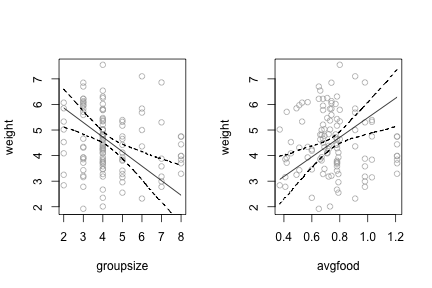
\includegraphics{weight-groupsize-avgfood} \begin{flushleft}
\ttfamily\noindent
\hspace*{\fill}\\
\hlstd{}\hlfunctioncall{par}\hlkeyword{(}\hlsymbol{op}\hlkeyword{)}\hspace*{\fill}\\
\hlstd{}\hspace*{\fill}\\
\hlstd{}\hlfunctioncall{precis}\hlkeyword{(}\hlsymbol{wgv.mle}\hlkeyword{)}\mbox{}
\normalfont
\end{flushleft}
\begin{verbatim}
##       Estimate Std. Error    2.5%   97.5%
## alpha   4.1232    0.43229  3.2759  4.9704
## b.g    -0.5687    0.15637 -0.8751 -0.2622
## b.v     3.8275    1.21306  1.4500  6.2051
## sigma   1.1166    0.07331  0.9729  1.2603
\end{verbatim}
\end{kframe}}
\end{knitrout}


The estimates are still awesome.
Tight CIs around the mean, clear evidence that as group size increases, weight decreases and that as avgfood increases so does weight. 


\subsection{(a)}


Finally, consider the avgfood variable. Fit two more multiple regres- sions: (1) body weight as an additive function of avgfood and group- size, and (2) body weight as an additive function of all three variables, avgfood and groupsize and area. Compare the results of these models to the previous models you’ve fit, in problems 1 and 2.
(a) Is avgfood or area a better predictor of body weight? If you had to choose one or the other to include in a model, which would it be? Support your assessment with any tables or plots you choose. In other words, you are on a long leash for this problem. I just want to see what you do.
(b) When both avgfood or area are in the same model, their effects are reduced (closer to zero) and their standard errors are larger than when they are included in separate models. Can you explain this re- sult?


\subsection*{Colophon}

\begin{knitrout}
\definecolor{shadecolor}{rgb}{.97, .97, .97}{\color{fgcolor}\begin{kframe}
\begin{flushleft}
\ttfamily\noindent
\hlfunctioncall{require}\hlkeyword{(}\hlsymbol{knitr}\hlkeyword{)}{\ }{\ }\hlcomment{\usebox{\hlnormalsizeboxhash}\usebox{\hlnormalsizeboxhash}\usebox{\hlnormalsizeboxhash}{\ }the{\ }package}\hspace*{\fill}\\
\hlstd{}\hlfunctioncall{knit}\hlkeyword{(}\hlfunctioncall{paste}\hlkeyword{(}\hlfunctioncall{getwd}\hlkeyword{(}\hlkeyword{)}\hlkeyword{,}{\ }\hlstring{"hw4ashander.Rnw"}\hlkeyword{,}{\ }\hlargument{sep}{\ }\hlargument{=}{\ }\hlstring{"/"}\hlkeyword{)}\hlkeyword{)}{\ }{\ }\hlcomment{\usebox{\hlnormalsizeboxhash}\usebox{\hlnormalsizeboxhash}{\ }to{\ }run}\mbox{}
\normalfont
\end{flushleft}
\end{kframe}}
\end{knitrout}



\end{document}
